% !TEX root = task-3-5-1.tex
% Editable task bank. Append new BankTask blocks at the end of the document.
\documentclass[12pt,a4paper]{article}
\usepackage{physics-textbook}
\usepackage{graphicx,needspace}
\usetikzlibrary{decorations.pathmorphing}
\newif\ifShowSolutions
\ifdefined\TutorEdition
  \ShowSolutionstrue
\else
  \ShowSolutionsfalse % Change to \ShowSolutionstrue to display solutions.
\fi
\newcounter{banktask}
\newsavebox{\BankTaskBox}
\newcommand{\BankTaskContent}[3]{%
  \noindent\textbf{\thebanktask.}\quad #2\par
  \ifShowSolutions
    \Needspace{50mm}% Keep the solution heading with its opening text or diagram.
    #3\par
    \ifdefined\TutorEdition
      \ifcsname TutorSource#1\endcsname
        \nopagebreak\smallskip{\small\csname TutorSource#1\endcsname\par}%
      \fi
    \fi
  \fi
}
\newcommand{\BankTask}[3]{%
  \refstepcounter{banktask}\par\medskip
  \sbox{\BankTaskBox}{\begin{minipage}{\linewidth}%
    \BankTaskContent{#1}{#2}{#3}\end{minipage}}%
  \ifdim\dimexpr\ht\BankTaskBox+\dp\BankTaskBox\relax>\dimexpr\textheight-20mm\relax
    \Needspace{35mm}\BankTaskContent{#1}{#2}{#3}%
  \else
    \Needspace{\dimexpr\ht\BankTaskBox+\dp\BankTaskBox\relax}%
    \noindent\usebox{\BankTaskBox}\par
  \fi
  \medskip
}
\begin{document}
\BookSubsection{3.5.1}{Поле внутри проводника}


% Source sdamgia-16857: https://phys-ege.sdamgia.ru/problem?id=16857
\BankTask{sdamgia-16857}{
На уединенной неподвижной проводящей сфере радиусом $R$ находится положительный заряд $Q$. Сфера находится в вакууме. Напряженность электростатического поля сферы в точке $A$ равна $36 \,\text{В/м}$. Все расстояния указаны на рисунке.\par
$1$. Потенциал электростатического поля в точке $A$ выше, чем в точке $F$: $\varphi_{A} > \varphi_{F}.$\par
$2$. Потенциал электростатического поля в точках $B$ и $D$ одинаков: $\varphi_{B} = \varphi_{D}.$\par
$3$. Потенциал электростатического поля в точках $A$ и $B$ одинаков: $\varphi_{A} = \varphi_{B}.$\par
$4$. Напряженность электростатического поля в точке $C$ $E_{C}=9 \,\text{В/м}$.\par
$5$. Напряженность электростатического поля в точке $B$ $E_{B}=0$.\par

\begin{center}\begin{tikzpicture}[book diagram,>=stealth]
\draw(0,0)circle(1.4);\draw(-.7,0)--(2.8,0)(0,0)--(0,-2.8);\foreach\x/\y/\label in{1.4/0/D,2.8/0/A,0/-1.4/F,0/-2.8/C}{\fill(\x,\y)circle(1.5pt);\node[above right]at(\x,\y){$\label$};}\fill(-.7,0)circle(1.5pt)node[above left]{$B$};\fill(0,0)circle(1.5pt);\draw[<->](-.7,0)--(0,0)node[midway,above]{$R/2$};\draw[<->](0,0)--(1.4,0)node[midway,above]{$R$};\draw[<->](1.4,0)--(2.8,0)node[midway,above]{$R$};\draw[<->](0,0)--(0,-1.4)node[midway,left]{$R$};\draw[<->](0,-1.4)--(0,-2.8)node[midway,left]{$R$};
\end{tikzpicture}\end{center}
\par
}{
\smallskip\noindent\textbf{Решение}\par
Для точечного заряда и поля снаружи заряженной сферы верны формулы: $\varphi = k \frac{ Q}{ r } ,E=k \frac{ Q}{ r ^2 } ,$ где $Q$ — величина точечного заряда или заряда сферы, $r$ — расстояние до точечного заряда или центра сферы. Потенциал на границе сферы равен потенциалу любой точки внутри сферы. Напряженность поля внутри сферы равна нулю.\par
Рассмотрим предложенные утверждения.\par
$1$. Расстояние от точки $A$ до центра сферы больше, чем расстояние от центра сферы до точки $F$, следовательно, потенциал в точке $F$ больше потенциала в точке $A$. Утверждение $1$ неверно.\par
$2$. Как известно из сказанного выше, потенциал внутри сферы равен потенциалу на границе сферы. Утверждение $2$ верно.\par
$3$. Потенциал в точке $B$ равен потенциалу на поверхности сферы, расстояние от точки $A$, до центра сферы больше радиуса сферы, следовательно, потенциал в точке $A$ меньше потенциала в точке $B$. Утверждение $3$ неверно.\par
$4$. Заметим, что точки $A$ и $C$ находятся на одинаковом расстоянии от центра сферы, следовательно, напряженности поля в этих точках равны и равны $36 \,\text{В/м}$. Утверждение $4$ неверно.\par
$5$. Как известно из сказанного выше, напряженность поля внутри сферы равна нулю. Утверждение $5$ верно.\par
Ответ: $25$.\par
}

% Source sdamgia-4577: https://phys-ege.sdamgia.ru/problem?id=4577
\BankTask{sdamgia-4577}{
На неподвижном проводящем уединенном шарике радиусом $R$ находится заряд $Q$. Точка О — центр шарика, $OA = \frac{ R}{ 2 } ,$ $OB = 4R$, $OC = 2R.$ Модуль напряженности электростатического поля заряда $Q$ в точке С равен $E_{\text{с}}.$ Чему равен модуль напряженности электростатического поля заряда $Q$ в точке $A$ и точке $B$?\par
Установите соответствие между физическими величинами и их значениями.\par

\begin{center}\begin{minipage}[t]{.47\linewidth}\textbf{Физические величины}\par\smallskip А) Модуль напряженности электростатического поля шарика в точке А \par
Б) Модуль напряженности электростатического поля шарика в точке В\end{minipage}\hfill\begin{minipage}[t]{.47\linewidth}\textbf{Их значения}\par\smallskip $1$) $0$\par
$2$) $4E_{c}$\par
$3$) $\frac{ E_{c}}{ 2 }$\par
$4$) $\frac{ E_{c}}{ 4 }$\end{minipage}\end{center}
\par
\begin{center}\small\setlength{\tabcolsep}{3pt}\begin{tabular}{|p{0.45\linewidth}|p{0.45\linewidth}|}\hline
$A$ & Б\\\hline
 & \\\hline
\end{tabular}\end{center}\par

\begin{center}\begin{tikzpicture}[book diagram,>=stealth]
\draw(0,0)circle(.8);\draw(-.3,0)--(3.2,0);\draw(0,0)--(-.8,-1.386);\foreach\x/\y/\s in{0/0/O,.4/0/A,3.2/0/B,-.8/-1.386/C}{\fill(\x,\y)circle(1.5pt);\node[above]at(\x,\y){$\s$};}
\end{tikzpicture}\end{center}
\par
}{
\smallskip\noindent\textbf{Решение}\par
Поскольку шар проводящий, весь заряд размещается на его поверхности, при этом электрическое поле внутри шара оказывается равным нулю (это называется экранировкой). Действительно, если бы поле было отлично от нуля, то оно привело бы к появлению тока внутри шара, но тока нет, и, значит, поле на самом деле равно нулю (А — $1$).\par
Снаружи от заряженного шара электрическое поле такое же, как от точечного заряда, помещенного в центр шара: $E= \frac{ kQ}{ r ^2 } .$ Точка $B$ отстоит от центра шара на вдвое большем расстоянии, чем точка С. Следовательно, напряженность поля в точке $B$ в $4$ раза меньше и равна $E_{c}/4$ (Б — $4$).\par
Ответ: $14$.\par
}

% Source sdamgia-4507: https://phys-ege.sdamgia.ru/problem?id=4507
\BankTask{sdamgia-4507}{
На неподвижном проводящем уединенном конусе высотой $H$ и радиусом основания $R= \frac{ H}{ 2 }$ находится заряд $Q$. Точка О — центр основания конуса, $AO = OC = 2R,$ $OB = R,$ угол АОС прямой, отрезки ОА и ОС лежат в плоскости основания конуса. Модуль напряженности электростатического поля заряда $Q$ в точке С равен $E_{\text{с}}.$ Чему равен модуль напряженности электростатического поля заряда $Q$ в точке А и точке В?\par
Установите соответствие между физическими величинами и их значениями.\par

\begin{center}\begin{minipage}[t]{.47\linewidth}\textbf{Физические величины}\par\smallskip А) Модуль напряженности электростатического поля конуса в точке А \par
Б) Модуль напряженности электростатического поля конуса в точке В\end{minipage}\hfill\begin{minipage}[t]{.47\linewidth}\textbf{Их значения}\par\smallskip $1$) $0$\par
$2$) $E_{c}$\par
$3$) $2E_{c}$\par
$4$) $4E_{c}$\end{minipage}\end{center}
\par
\begin{center}\small\setlength{\tabcolsep}{3pt}\begin{tabular}{|p{0.45\linewidth}|p{0.45\linewidth}|}\hline
$A$ & Б\\\hline
 & \\\hline
\end{tabular}\end{center}\par

\begin{center}\begin{tikzpicture}[book diagram,>=stealth]
\draw(0,0)ellipse(1.5 and .6);\draw(-1.5,0)--(0,3)--(1.5,0);\draw(0,3)--(0,0)--(-3,0);\draw(0,0)--(-1.5,-1.5);\foreach\x/\y/\s in{0/1.5/B,-3/0/A,-1.5/-1.5/C}{\fill(\x,\y)circle(1.5pt);\node[below left]at(\x,\y){$\s$};}
\fill(0,0)circle(1.5pt);\node[right]at(0,0){$O$};\end{tikzpicture}\end{center}
\par
}{
\smallskip\noindent\textbf{Решение}\par
Поскольку конус проводящий, весь заряд размещается на его поверхности, при этом электрическое поле внутри конуса оказывается равным нулю (это называется экранировкой). Действительно, если бы поле было отлично от нуля, то оно привело бы к появлению тока внутри конуса, но тока нет, и, значит, поле на самом деле равно нулю (Б — $1$).\par
Конус представляет собой систему с осевой симметрией. Из соображений симметрии заключаем, что распределение заряда на конусе и создаваемое этим зарядом электрическое поле так же обладают данным свойством. А значит, модуль напряженности электростатического поля конуса в точке А равен $E_{c}$ ($A$ — $2$).\par
Ответ: $21$.\par
}

% Source sdamgia-31415: https://phys-ege.sdamgia.ru/problem?id=31415
\BankTask{sdamgia-31415}{
Стеклянные незаряженные кубики~$1$ и $2$ и алюминиевые незаряженные кубики~$3$ и $4$ сблизили вплотную и поместили в электрическое поле, напряженность которого направлена горизонтально влево, как показано в левой части рисунка. Затем кубики раздвинули и уже после этого выключили электрическое поле (правая часть рисунка).\par
$1$. В электрическом поле (левая часть рисунка) часть электронов перешла из кубика~$4$ в кубик~$3$.\par
$2$. Кубик $2$, изображенный в правой части рисунка, не заряжен.\par
$3$. В электрическом поле (левая часть рисунка) правая грань кубика~$2$ заряжена положительно.\par
$4$. Кубик $3$, изображенный в правой части рисунка, имеет положительный заряд.\par
$5$. В электрическом поле (левая часть рисунка) разность потенциалов между левой гранью кубика~$3$ и правой гранью кубика~$4$ равна нулю.\par

\begin{center}\begin{tikzpicture}[book diagram,>=stealth]
\draw(0,0)rectangle(1.2,1.2);\draw(.6,0)--(.6,1.2)(0,.6)--(1.2,.6);\foreach\x/\y/\s in{.3/.9/1,.9/.9/2,.3/.3/3,.9/.3/4}\node at(\x,\y){$\s$};\foreach\y in{.3,.5,.7,.9}\draw[->](-.2,\y)--(-1,\y);\node[above]at(-.7,1){$\vec E$};\draw[dashed](1.65,-.2)--(1.65,1.4)(1.8,-.2)--(1.8,1.4);\foreach\x/\y/\s in{2.1/.8/1,3.1/.8/2,2.1/-.2/3,3.1/-.2/4}{\draw(\x,\y)rectangle++(.6,.6);\node at(\x+.3,\y+.3){$\s$};}
\end{tikzpicture}\end{center}
\par
}{
\smallskip\noindent\textbf{Решение}\par
$1$. Неверно. Электроны под действием электрического поля движутся против силовых линий, поэтому переместятся вправо, тогда часть электронов перейдет с кубика~$3$ в кубик~$4$.\par
$2$. Верно. Стекло является диэлектриком, в котором нет свободных носителей заряда. Поэтому кубики из стекла останутся незаряженными.\par
$3$. Неверно. В кубиках из стекла произойдет поляризация, в результате которой правая часть кубика~$2$ будет иметь отрицательный заряд.\par
$4$. Верно. Поскольку электроны в металлах переместятся против силовых линий, то в кубике~$3$ будет недостаток электронов, он будет заряжен положительно.\par
$5$. Верно. В проводнике, помещенном в электростатическое поле, напряженность станет равной $0$, поэтому и разность потенциалов между левой гранью кубика~$3$ и правой гранью кубика~$4$ равна нулю.\par
Ответ: $245$.\par
}

% Source sdamgia-6431: https://phys-ege.sdamgia.ru/problem?id=6431
\BankTask{sdamgia-6431}{
В нижней половине незаряженного металлического шара находится крупная шарообразная полость, заполненная воздухом. Шар находится в воздухе вдали от других предметов. В центр полости помещен положительный точечный заряд $q > 0$ (см. рис.). Нарисуйте картину силовых линий электростатического поля внутри полости и снаружи шара. Если поле равно нулю, напишите в данной области: $\vec{E}=0.$ Если поле отлично от нуля, нарисуйте картину поля в данной области, используя восемь силовых линий.\par

\begin{center}\begin{tikzpicture}[book diagram,>=stealth]
\draw[fill=gray!12](0,0)circle(1.5);\draw[fill=white](0,-.5)circle(.75);\fill(0,-.5)circle(1.5pt);\node[below right]at(0,-.5){$q$};
\end{tikzpicture}\end{center}
\par
}{
\smallskip\noindent\textbf{Решение}\par

\begin{center}\begin{tikzpicture}[book diagram,>=stealth]
\draw[fill=gray!12](0,0)circle(1.5);\draw[fill=white](0,-.5)circle(.75);\node at(0,.8){$E=0$};\foreach\a in{0,45,...,315}{\draw[->](\a:1.5)--(\a:2.3);\draw[->](0,-.5)--++(\a:.72);}
\end{tikzpicture}\end{center}
\par
$1$. Приведен схематический рисунок картины силовых линий: внутри полости — семейство прямых лучей, исходящих из заряда и приходящих на поверхность полости по нормали; снаружи шара — семейство прямых лучей, исходящих с поверхности шара по нормали к ней и уходящих на бесконечность.\par
$2$. Внутри проводника — электростатическое поле $E=0.$ Поэтому поле в полости обладает центральной симметрией и выглядит как поле точечного заряда $q > 0,$ находящегося в центре полости. Силовые линии этого поля подходят по нормали к поверхности полости, где равномерно распределен отрицательный индуцированный заряд $-q < 0.$\par
$3$. На наружной поверхности шара находится (в силу нейтральности шара в целом) положительный заряд $q > 0.$ В силу того, что внутри проводника $\vec{E}=0,$ а снаружи окружающие предметы расположены далеко от шара, этот заряд распределен по поверхности шара равномерно. Его поле вне шара выглядит как поле точечного заряда $q > 0,$ расположенного в центре шара. Силовые линии отходят от шара по нормали к его поверхности.\par
}

% Source sdamgia-4218: https://phys-ege.sdamgia.ru/problem?id=4218
\BankTask{sdamgia-4218}{
Внутри незаряженного металлического шара радиусом $r_{1}=40 \,\text{см}$ имеются две сферические полости радиусами $r_{2} < \frac{ r_{1}}{ 2 } ,$ расположенные таким образом, что их поверхности почти соприкасаются в центре шара. В центре одной полости поместили заряд $q_{1}= + 1\,\text{нКл}$, а затем в центре другой — заряд $q_{2}= + 2\,\text{нКл}$ (см. рис.). Найдите модуль и направление вектора напряженности $\vec{E}$ электростатического поля в точке $O$, находящейся на расстоянии $R=1 \,\text{м}$ от центра шара на перпендикуляре к отрезку, соединяющему центры полостей.\par

\begin{center}\begin{tikzpicture}[book diagram,>=stealth]
\draw[fill=gray!12](0,0)circle(1.5);\draw[fill=white](0,.67)circle(.67)(0,-.67)circle(.67);\draw(-1.5,0)--(2.7,0);\draw(0,.67)--(0,-.67);\draw(0,0)--(.14,0)--(.14,.14)--(0,.14);\foreach\y/\s in{.67/q_1,-.67/q_2}{\fill(0,\y)circle(1.5pt);\node[right]at(0,\y){$\s$};}\fill(2.7,0)circle(1.5pt)node[above right]{$O$};\node[above]at(-.85,0){$r_1$};\node[left]at(0,.35){$r_2$};\node[left]at(0,-.35){$r_2$};\node[above]at(1.9,0){$R$};
\end{tikzpicture}\end{center}
\par
}{
\smallskip\noindent\textbf{Решение}\par
Возможное решение\par
В электростатике считается, что электрическое поле внутри металла отсутствует, так как иначе свободные заряды внутри металла двигались бы. Поэтому при помещении заряда $q_{1}$ в первую полость на ее стенках индуцируется заряд $- q_{1}$ и по принципу суперпозиции суммарное поле этих двух зарядов в металле шара равно нулю. По закону сохранения электрического заряда и в силу электронейтральности шара избыточный заряд равен $q_{1}.$ Он вытесняется на поверхность шара и равномерно распределяется по ней, так как заряды внутри металла не создают поля и не влияют на распределение зарядов на поверхности шара.\par
После помещения заряда $q_{2}$ во вторую полость все происходит аналогичным образом, и на поверхность шара вытесняется дополнительно заряд $q_{2},$ так что теперь на поверхности шара равномерно распределяется суммарный заряд $q_{1} + q_{2}.$\par
Поле равномерно заряженного шара вне его совпадает с полем точечного заряда, помещенного в центр шара, поэтому поле в точке $O$, находящейся на расстоянии $R$ от центра шара, по модулю равно $E= \frac{ 1}{ 4 \pi \varepsilon _{0} } \cdot \frac{ q_{1} + q_{2}}{ R ^2 } =27\,\text{В/м}$ и направлено вдоль радиуса от центра шара к точке $O.$\par
Здесь $\varepsilon _{0}$ — электрическая постоянная.\par
Ответ: $E=27\,\text{В/м}$, вектор $\vec{E}$ направлен от центра шара к точке $O.$\par
}


% Source 896222: https://ege.fipi.ru/bank/questions.php?search=1&proj=BA1F39653304A5B041B656915DC36B38&qid=896222
\BankTask{896222}{
Незаряженное металлическое тело, продольное сечение которого показано на рисунке, поместили в однородное электрическое поле напряжённостью $\vec{E}$.

Какие два утверждения описывают результаты воздействия этого поля на металлическое тело?
\begin{enumerate}
\item Напряжённость электрического поля в точке $D$ равна нулю.
\item Потенциалы в точках $B$ и $C$ равны.
\item Концентрация свободных электронов в точке $A$ наибольшая.
\item В точке $A$ индуцируется положительный заряд.
\item В точке $D$ индуцируется отрицательный заряд.
\end{enumerate}
\begin{center}
\begin{tikzpicture}[book diagram,x=1cm,y=1cm]

\draw[-{book tip}] (0,2.45)--(3.8,2.45);
\draw[-{book tip}] (0,0.15)--(3.8,0.15);
\node[above] at (3.6,2.55) {$\vec E$};
\node[above] at (3.6,0.25) {$\vec E$};
\draw[fill=gray!55,line width=0.6pt] (0.85,0.87)--(3.05,0.87) arc[start angle=-90,end angle=90,radius=0.45]--(0.85,1.77) arc[start angle=90,end angle=270,radius=0.45]--cycle;
\fill (1.95,1.77) circle (0.035);
\fill (0.4,1.32) circle (0.035);
\fill (3.5,1.32) circle (0.035);
\fill (1.95,1.36) circle (0.04);
\node[above] at (1.95,1.82) {$A$};
\node[left] at (0.4,1.32) {$B$};
\node[right] at (3.5,1.32) {$C$};
\node[right] at (1.97,1.3) {$D$};
\end{tikzpicture}
\end{center}
}{
\smallskip\noindent\textbf{Решение от GPT}\par
В электростатическом равновесии внутри металла $\vec E=0$, а весь проводник эквипотенциален: $\varphi_B=\varphi_C$; утверждения 1 и 2 верны. Электроны смещаются против внешнего поля и накапливаются у левого края $B$, поэтому утверждение 3 неверно. В точке $A$ на середине боковой поверхности положительный заряд не индуцируется, а внутри металла в точке $D$ избыточного заряда нет, поэтому утверждения 4 и 5 неверны. Ответ: $12$.
}

% Source 29998: https://phys-ege.sdamgia.ru/problem?id=29998
\BankTask{29998}{
\begin{center}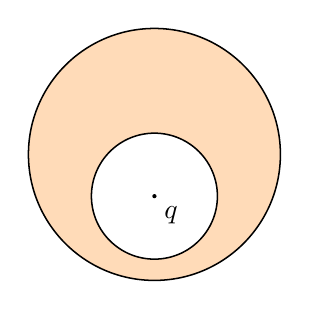
\begin{tikzpicture}[>=stealth,line width=.55pt]\draw[fill=orange!28](0,0)circle(1.6);\draw[fill=white](0,-.53)circle(.8);\fill(0,-.53)circle(.027)node[below right]{$q$};\end{tikzpicture}\end{center}В нижней половине незаряженного металлического шара располагается крупная шарообразная полость, заполненная воздухом. Шар находится в воздухе вдали от других предметов. В центр полости помещен положительный точечный заряд q > $0$ (см. рисунок). Нарисуйте картину линий напряженности электростатического поля внутри полости, внутри проводника и снаружи шара. Если поле отсутствует, напишите в данной области: $\vec{E} = 0.$ Если поле отлично от нуля, нарисуйте картину поля в данной области, используя восемь линий напряженности. Ответ поясните, указав, какие физические закономерности Вы использовали для объяснения.
}{
\smallskip\noindent\textbf{Решение}\par
\begin{center}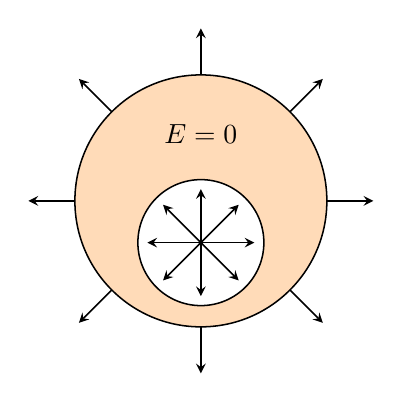
\begin{tikzpicture}[>=stealth,line width=.55pt]\draw[fill=orange!28](0,0)circle(1.6);\draw[fill=white](0,-.53)circle(.8);\node at(0,.85){$E=0$};\foreach \a in {0,45,...,315}{\draw[->](\a:1.6)--(\a:2.19);\draw[->](0,-.53)--++(\a:.68);}\fill(0,-.53)circle(.03);\end{tikzpicture}\end{center}$1$.  Приведен схематический рисунок картины линий напряженности: внутри полости  — семейство прямых лучей, исходящих из заряда и приходящих на поверхность полости по нормали; снаружи шара  — семейство прямых лучей, по нормали к ней и уходящих в бесконечность. 
$2$.  Внутри проводника  — электростатическое поле $\vec{E}=0.$ 
$3$.  Заряд q помещен в центр шарообразной полости, поэтому его электростатическое поле в полости обладает центральной симметрией и выглядит как поле уединенного точечного заряда $q > 0,$ находящегося в центре полости. Линии напряженности этого поля подходят по нормали к поверхности полости, где равномерно распределен отрицательный индуцированный заряд $- q < 0.$ 
$4$.  На наружной поверхности шара находится (в силу нейтральности шара в целом) положительный заряд $q > 0.$ Поскольку внутри проводника $\vec{E}=0,$ а снаружи окружающие предметы расположены далеко от шара, этот заряд распределен по поверхности шара равномерно. Его поле вне шара выглядит как поле уединенного точечного заряда q > $0$, расположенного в центре шара. Линии напряженности отходят от шара по нормали к его поверхности.
}

\end{document}
